%%%%%%%%%%%%%%%%%%%%%%%%%%%%%%%%%%%%%%%%
%%%%%  xPhO LaTeX Beamer Template  %%%%%
%%%%%  Date: 17/03/2025            %%%%%
%%%%%  Authors:                    %%%%%
%%%%%       Nguyen Thanh Long      %%%%%
%%%%%       Nguyen Le Mai Huong    %%%%%
%%%%%       Nguyen Minh Phuong     %%%%%
%%%%%%%%%%%%%%%%%%%%%%%%%%%%%%%%%%%%%%%%

\documentclass[aspectratio=169, t]{beamer} % Ratio 16:9
\usepackage[T5]{fontenc}
\usepackage{lmodern}
\usepackage{graphicx} 
\usepackage{array}
\usepackage{longtable} % for long table
\usepackage{chngcntr}
\counterwithin{figure}{section}
\usepackage{tcolorbox}
\renewcommand{\familydefault}{\sfdefault} % Font

\usepackage{caption}
\usepackage{subcaption}
\usepackage{siunitx}

% \definecolor{BlueDefault}{rgb}{0.2,0.2,0.7}
\definecolor{BlueDefault}{RGB}{14,47,95}


% Hide navigation 
\setbeamertemplate{navigation symbols}{}

% Setup background
\newcommand{\normalbackground}{%
    \usebackgroundtemplate{
\includegraphics[width=\paperwidth,height=\paperheight]{Slides/Background/Normal_slide_xPhO.pdf}}%
}

\newcommand{\titlebackground}{%
    \usebackgroundtemplate{
\includegraphics[width=\paperwidth,height=\paperheight]{Slides/Background/Title_slide_xPhO.pdf}}%
}

% Change the title color to white
\setbeamercolor{frametitle}{fg=white} 

% push the title up by \raisebox
\setbeamertemplate{frametitle}{%
    \vspace{0.3em}
    \hspace{-1em} \insertframetitle
    \vspace{2mm}
}

% Number of slide
\setbeamertemplate{footline}{%
    \hfill
    \insertframenumber/\inserttotalframenumber
    \hspace{7.5mm}
    \vspace{3.5mm}
}

%% Make Table of Contents %%
\AtBeginSection[]{
  \begin{frame}
  \frametitle{Mục lục}
  \tableofcontents[currentsection]
  \end{frame}
}

%% Section numbering %%
\setbeamertemplate{section in toc}[sections numbered]
\setbeamertemplate{subsection in toc}[subsections numbered]


\renewcommand{\figurename}{Hình}
\renewcommand{\tablename}{Bảng}


%%%%% Bibliography %%%%%
\usepackage[backend=biber,style=ieee]{biblatex}
\addbibresource{citation.bib}

\usepackage{url}
\usepackage{hyperref}
\hypersetup{
	colorlinks=true,
	linkcolor=BlueDefault,
	filecolor=BlueDefault,
    citecolor=BlueDefault,
	urlcolor=BlueDefault,
	pdftitle={Overleaf Example},
	pdfpagemode=FullScreen,
}

\begin{document}

\titlebackground

\begin{frame}[noframenumbering]
    \thispagestyle{empty}
    \bfseries
    \begin{flushleft}
        \vfill
        \vspace{5mm}
        \textcolor{BlueDefault}{\huge \bfseries Vector và  \\Nhập môn Đại số tuyến tính} \\
        \vspace{8mm}
        \textcolor{black}{\large \bfseries Người trình bày: Carina }
        \vfill
    \end{flushleft}
\end{frame}

\normalbackground


\section{Mở đầu về giải tích}
\subsection{Tốc độ }
\begin{frame}
\frametitle{Tốc Độ}
Tốc độ trung bình: 
\[\overline{v}=\frac{\Delta s}{\Delta t}.\]
Đo tốc độ:
\begin{itemize}
    \item Quãng đường 
    \item Thời gian 
    \item Sai số
\end{itemize}
\vspace{8pt}

Sai số của phép đo ứng với: \(1000\text{m}\rightarrow 1\text{m}\rightarrow 1\text{cm}.\)

Ví dụ: Thời gian đi hết 1cm của một người đang chạy.
\end{frame}
\begin{frame}
\frametitle{Vai trò của giải tích}
     Sự cần thiết của một đại lượng:
     \begin{itemize}
        \item Có thể tính được (dựa trên mô hình toán học)
        \item Thuần tuý toán học (không bị ràng buộc bởi thực nghiệm)
        \item Phản ảnh quy luật chuyển động của vật
     \end{itemize}
     \vspace{8pt}

     \(\implies \text{Tốc độ tức thời và Giải tích}\)
\end{frame}
\subsection{Sơ lược lịch sử}
\begin{frame}
\frametitle{Giới thiệu}
\begin{figure}[htbp]
    \centering
    % Ảnh bên trái
    \begin{subfigure}[t]{0.45\textwidth}
        \centering
        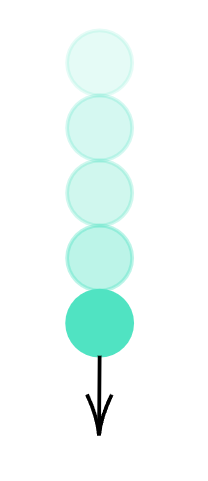
\includegraphics[width=2cm, height=3cm]{Slides/figure/free fall.png}
        \caption{Rơi tự do}
    \end{subfigure}
    \hfill
    % Ảnh bên phải
    \begin{subfigure}[t]{0.45\textwidth}
        \centering
        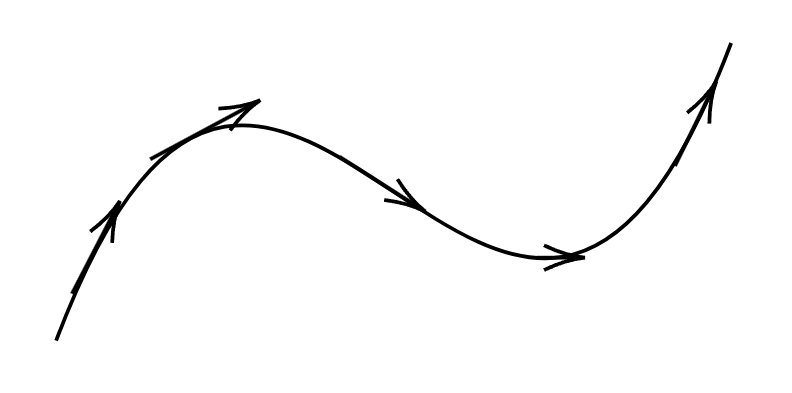
\includegraphics[width=3cm, height=2cm]{Slides/figure/curvature.png}
        \caption{Một đường cong}
    \end{subfigure}
    \caption{Hai thay đổi điển hình-thời gian,và hướng.}
\end{figure}
Giải tích là toán học nghiên cứu sự thay đổi.
\end{frame}
\begin{frame}
\frametitle{Sơ lược lịch sử}
    \begin{figure}[htbp]
    \centering
    % Ảnh bên trái
    \begin{subfigure}[t]{0.45\textwidth}
        \centering
        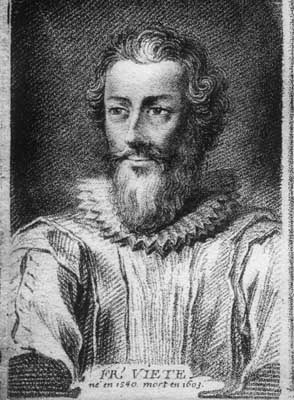
\includegraphics[width=4cm, height=5cm]{Slides/figure/Francois_Viete.jpeg}
        \caption{Francois Viete (1540-1603)}
    \end{subfigure}
    \hfill
    % Ảnh bên phải
    \begin{subfigure}[t]{0.45\textwidth}
        \centering
        \includegraphics[width=4cm, height=5cm]{Slides/figure/Frans_Hals_-_Portret_van_René_Descartes.jpg}
        \caption{René Descartes (1596-1650)}
    \end{subfigure}
    \caption{Sự phát triển của đại số  và hình học giải tích.}
\end{figure}
\end{frame}
\begin{frame}
\frametitle{Sơ lược lịch sử}    
     \begin{figure}[htbp]
    \centering
    % Ảnh bên trái
    \begin{subfigure}[t]{0.45\textwidth}
        \centering
        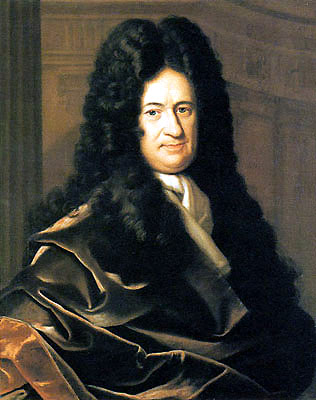
\includegraphics[width=4cm, height=5cm]{Slides/figure/Gottfried_Wilhelm_von_Leibniz.jpg}
        \caption{G.W.Leibniz (1646-1716)}
    \end{subfigure}
    \hfill
    % Ảnh bên phải
    \begin{subfigure}[t]{0.45\textwidth}
        \centering
        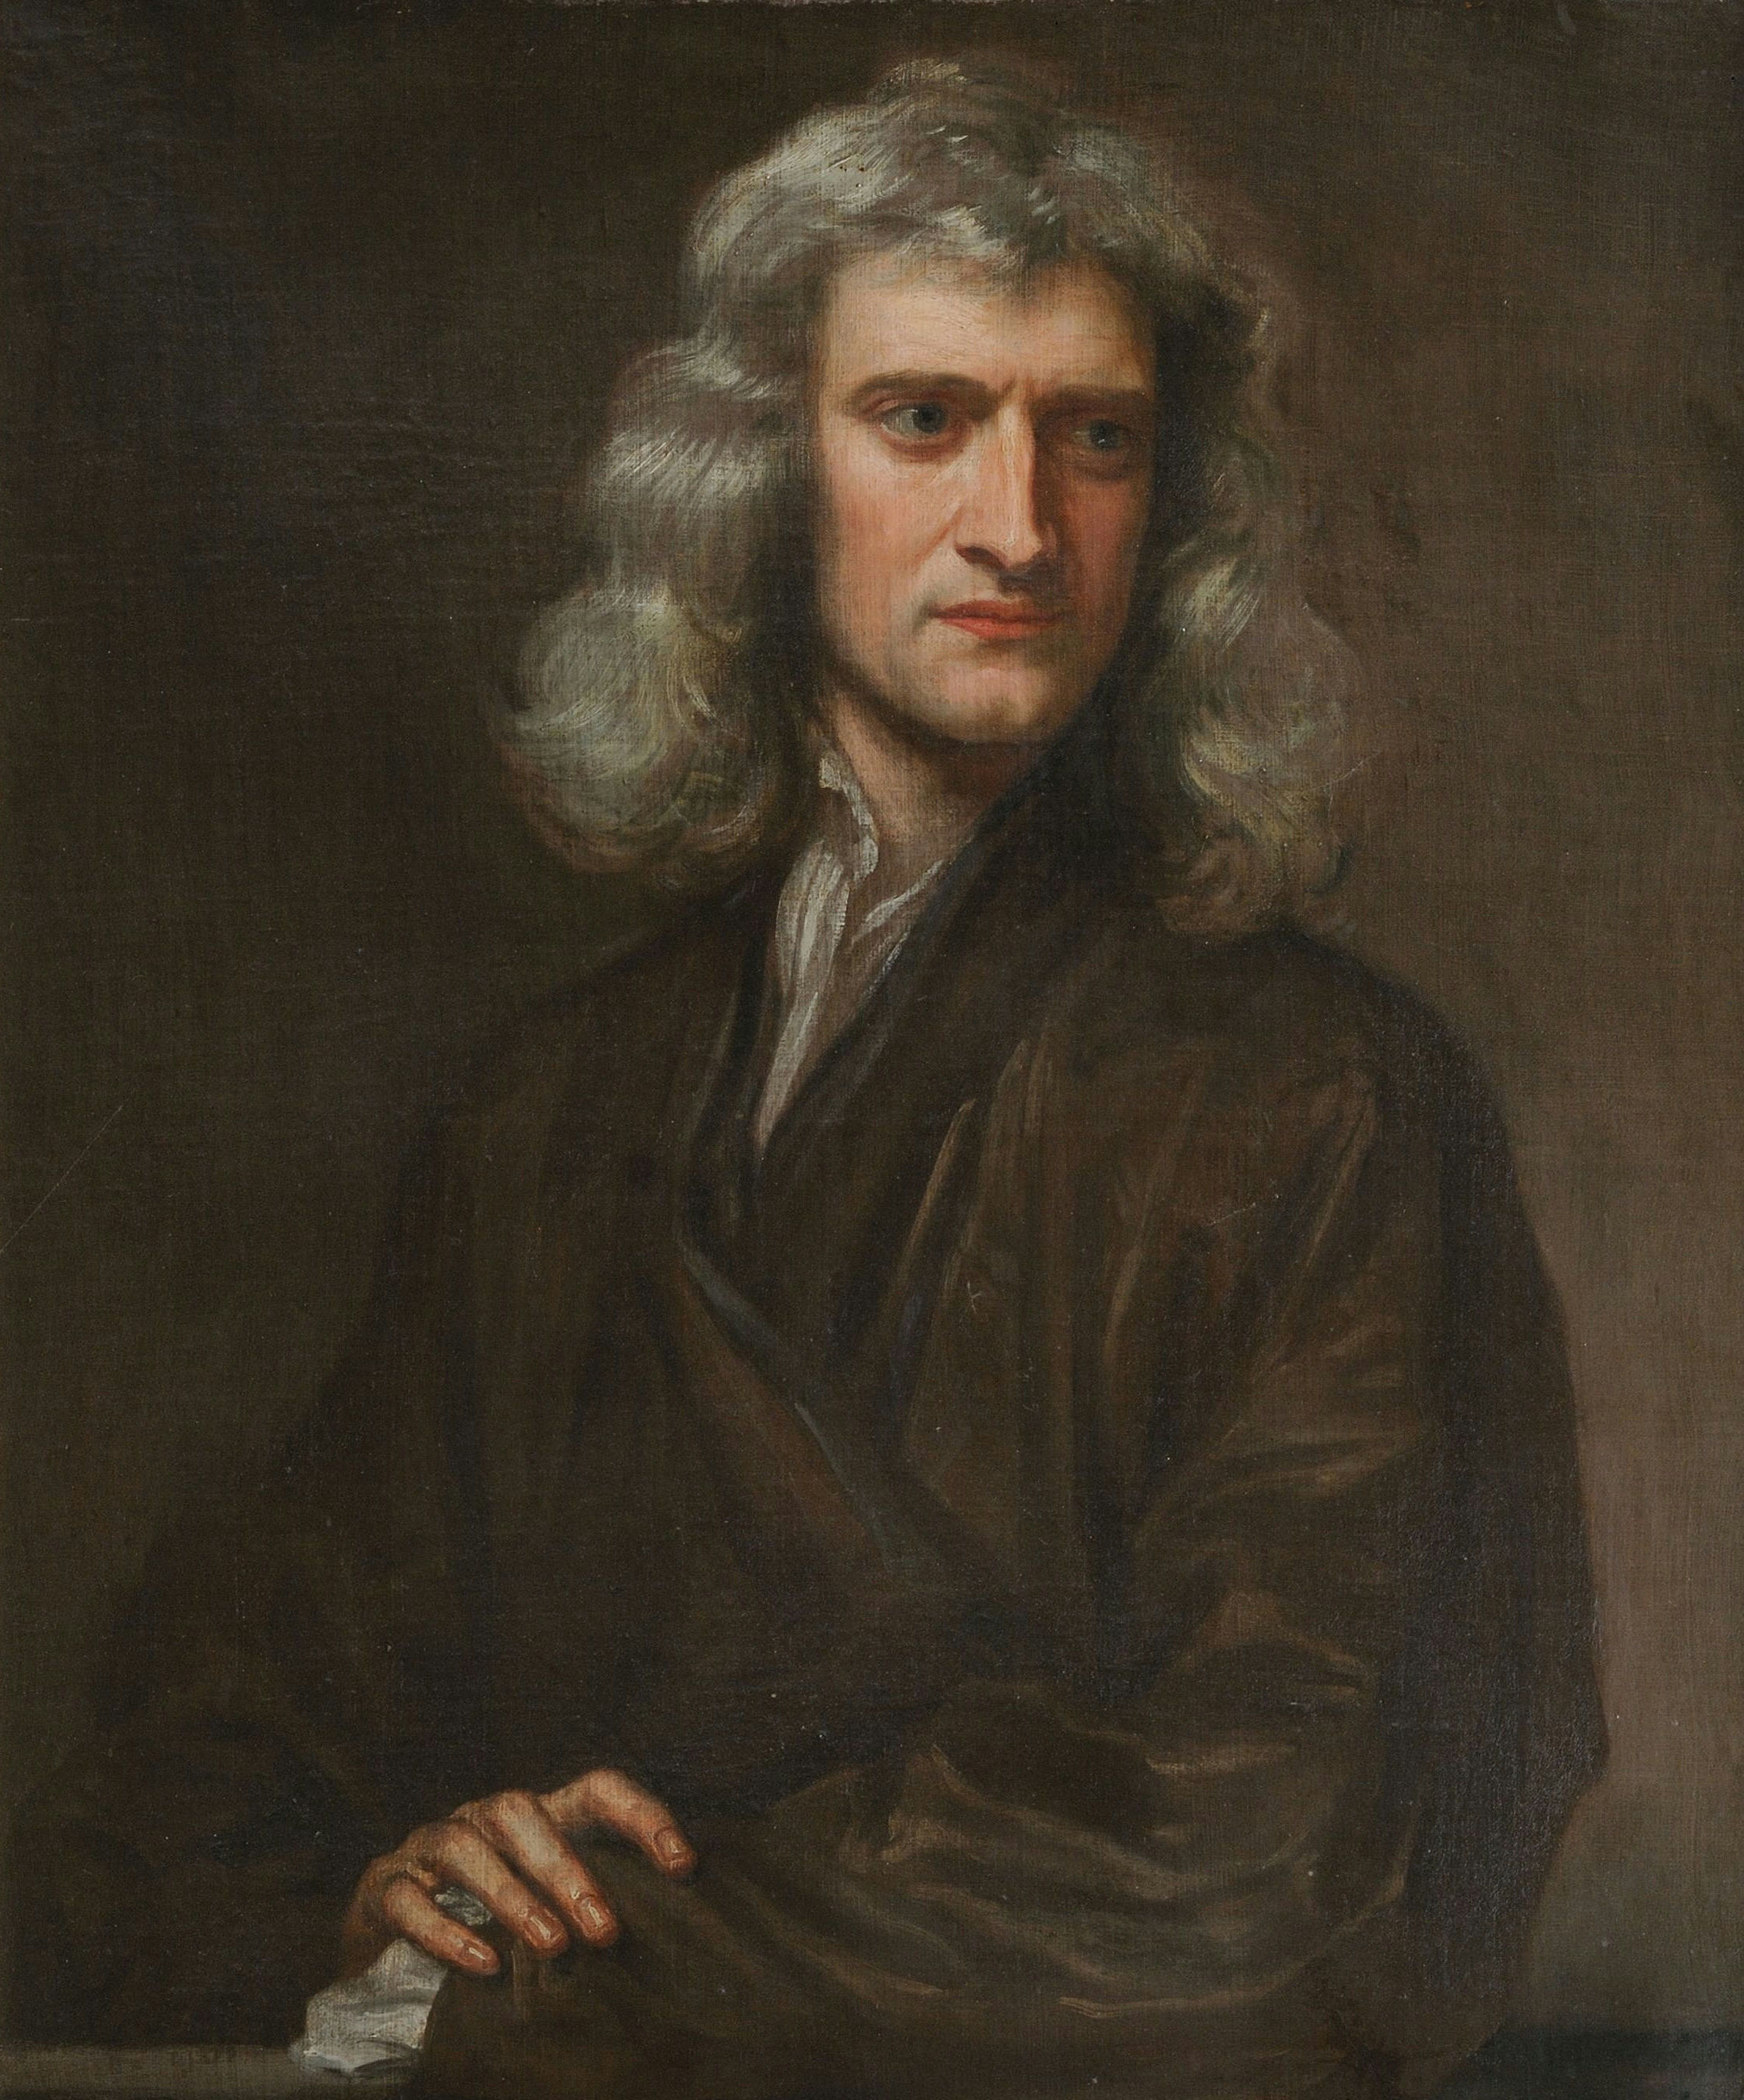
\includegraphics[width=4cm, height=5cm]{Slides/figure/Portrait_of_Sir_Isaac_Newton,_1689.jpg}
        \caption{Isaac Newton (1642-1727)}
    \end{subfigure}
\end{figure}
\end{frame}

\begin{frame}{Hình học giải tích}
    \begin{figure}[htbp]
    \centering
    % Ảnh bên trái
    \begin{subfigure}[t]{0.45\textwidth}
        \centering
        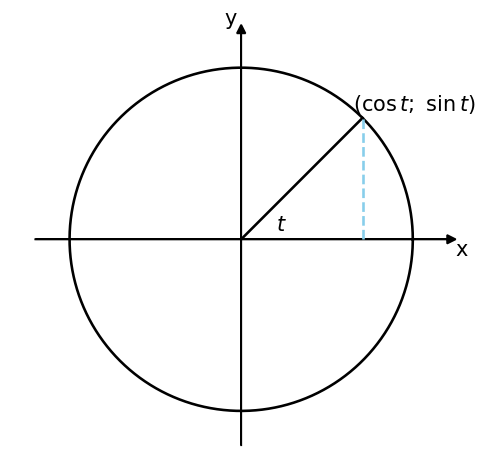
\includegraphics[width=3.5cm, height=3cm]{Slides/figure/duongtronthamso - Copy.png}
    \end{subfigure}
    \hfill
    % Ảnh bên phải
    \begin{subfigure}[t]{0.45\textwidth}
        \centering
        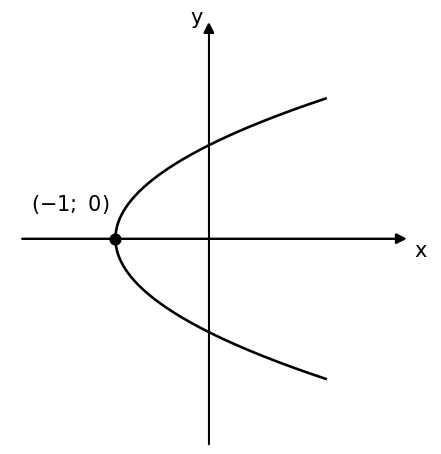
\includegraphics[width=3.5cm, height=3cm]{Slides/figure/parabolngang - Copy.png}
    \end{subfigure}
    \hfill
    \begin{subfigure}[t]{0.45\textwidth}
        \centering
        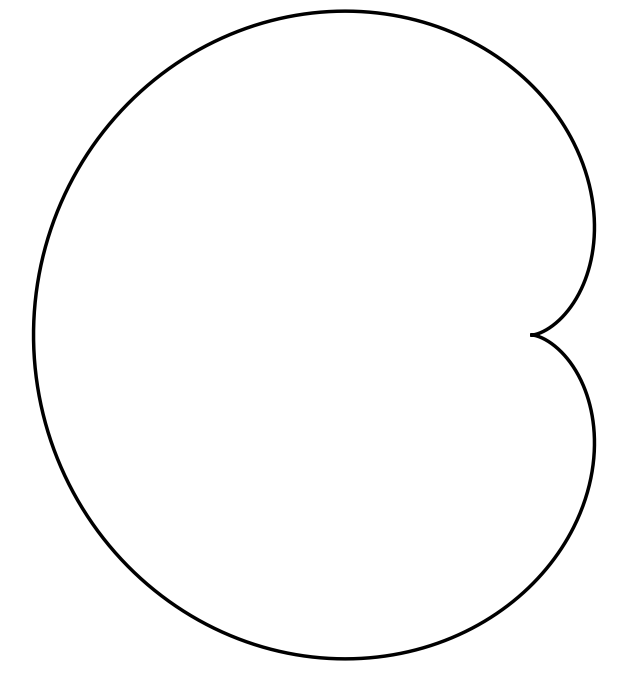
\includegraphics[width=3cm, height=3cm]{Slides/figure/cardioid - Copy.png}
    \end{subfigure}
    \hfill
    \begin{subfigure}[t]{0.45\textwidth}
        \centering
        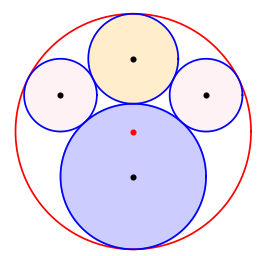
\includegraphics[width=3cm, height=3cm]{Slides/figure/4circle.png}
    \end{subfigure}
\end{figure}
\end{frame}
\section{Hàm số và Đồ thị}
% Add this to your preamble (at the top of your .tex file, before \begin{document}):
% \usepackage{subcaption}
% \usepackage{float}

\begin{frame}
\frametitle{Hàm số và Đồ thị}
    \begin{tcolorbox}[colback=blue!10!, colframe=blue!50!black, title=Định nghĩa]
        \textit{Hàm} $f$ là một quy tắc cho tương ứng mỗi phần tử x thuộc tập hợp $X$ với một và chỉ một phần tử , kí hiệu $f(x)$, thuộc một tập hợp $Y$.
    \end{tcolorbox}
     \begin{figure}
      \centering
      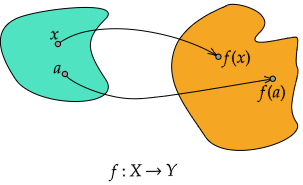
\includegraphics[width=6cm, height= 3cm]{Slides/figure/anhxa - Copy.png}
     \end{figure}
\end{frame}

\begin{frame}
\frametitle{Hàm số và Đồ thị}
   Đồ thị của \(f\) bao gồm mọi điểm \((x,y)\) sao cho \(y=f(x)\) với \(x\in X\).
  \begin{columns}
    \begin{column}{0.5\textwidth}
      \begin{figure}
        \centering
        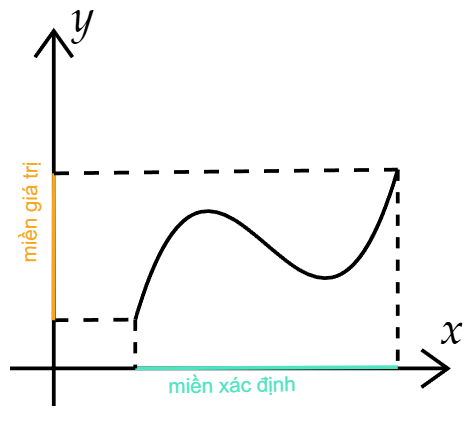
\includegraphics[width=5cm, height= 4cm]{Slides/figure/hamso1 - Copy.png}
      \end{figure}
    \end{column}
    \begin{column}{0.5\textwidth}
      Một số hàm số quen thuộc:
      \begin{itemize}
        \item \(y=\sin x : X= (-\infty, \infty), Y=[-1,1]\)
        \item \(y=\lvert x\rvert : X= (-\infty, \infty), Y=(0,\infty)\)
      \end{itemize}
      Chú ý, đây không phải là một hàm số:
    \begin{figure}
        \centering
        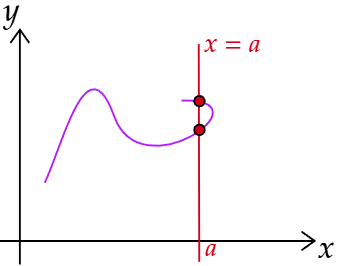
\includegraphics[width=4cm, height= 3cm]{Slides/figure/khongphaihamso - Copy.png}
      \end{figure}
    \end{column}
  \end{columns}
\end{frame}
     
\section{Đạo hàm}
\begin{frame}{Đạo hàm}
    \begin{tcolorbox}[colback=blue!10, colframe=blue!50!black, title=Định nghĩa]
    \textbf{Đạo hàm} của hàm số $f$ tại giá trị $a$, kí hiệu bởi $f'(a)$, là
    \begin{equation}
        f'(a)=\lim_{\Delta x\rightarrow 0}\dfrac{f(a+\Delta x)-f(a)}{\Delta x}
    \end{equation}
    nếu giới hạn này tồn tại.
    \end{tcolorbox}
\end{frame}
\begin{frame}{Đạo hàm}
    \textbf{Các định lý của đạo hàm:}
\begin{tcolorbox}[colback=blue!10, colframe=blue!50!black, title=Định lý]
Nếu $f$ khả vi tại $a$, thì $f$ liên tục tại $a$.
\end{tcolorbox}
\textit{Lưu ý: Mệnh đề đảo của định lý này là sai, có các hàm liên tục khưng không khả vi. Ví dụ, hàm $f(x)=|x|$ là hàm liên tục nhưng không khả vi.}
\end{frame}
\begin{frame}{Đạo hàm}
\begin{tcolorbox}[colback=blue!10, colframe=blue!50!black, title=Định lý]
Nếu $f$ và $g$ khả vi
$$
    (f\pm g)'=f'\pm g',\quad (fg)'=f'g+g'f,\quad \left(\dfrac{f}{g}\right)'=\dfrac{f'g+g'f}{g^2}\text{ với }g(x)\neq 0.
$$
\end{tcolorbox}
\end{frame}
\begin{frame}{Đạo hàm}
    \begin{tcolorbox}[colback=blue!10, colframe=blue!50!black, title=Định lý đạo hàm hợp]
    Nếu $g$ khả vi tại $x$ và $f$ khả vi tại $g(x)$, thì hàm hợp $F=f\circ g\equiv f(g(x))$ khả vi tại $x$ và $F'$ được xác định bởi tích
    \begin{equation}
        F'(x)=f'(g(x))\dot g'(x)
    \end{equation}
    Theo ký hiệu của Leibniz, nếu $y=f(u)$ và $u=g(x)$ đều là hàm khả vi, thì
    \begin{equation}
        \dfrac{dy}{dx}=\dfrac{dy}{du}\dfrac{du}{dx}
    \end{equation}
    \end{tcolorbox}
\end{frame}
\begin{frame}
    \frametitle{Tiếp tuyến và tốc độ biến thiên}
  Xét đường cát tuyến của đường cong có phương trình $y=f(x)$ đi qua 2 điểm $P(a, f(a))$ và $Q(x, f(x))$ với $x\neq a$. Hệ số góc của đường cát tuyến PQ:
  \begin{equation}
      m_{PQ}=\dfrac{f(x)-f(a)}{x-a}
  \end{equation}
  \textit{(Hình vẽ)}
  \end{frame}
  \begin{frame}
  {Tiếp tuyến và tốc độ biến thiên}
  \begin{tcolorbox}[colback=blue!10, colframe=blue!50!black, title=Định nghĩa]
  \textbf{Tiếp tuyến} của đường cong $y=f(x)$ tại điểm $P(a, f(a)$ là đường thẳng đi qua $P$ với hệ số góc
  \begin{equation}
      m=\lim_{x\rightarrow a}\dfrac{f(x)-f(a)}{x-a}=f'(a)
  \end{equation}
  Nếu giới hạn này tồn tại.
  \end{tcolorbox}
  \begin{tcolorbox}[colback=blue!10, colframe=blue!50!black, title= ]
  Đạo hàm $f'(a)$ chính là hệ số góc của đường tiếp tuyến của đường cong $y=f(x)$ tại $x=a$.
  \end{tcolorbox}
    \end{frame}
  \begin{frame}{Tiếp tuyến và tốc độ biến thiên}
      Giả sử $y$ là đại lượng phụ thuộc vào một đại lượng khác $x$. Khi đó ta viết $y=f(x)$. Nếu $x$ biến thiên từ $x_1$ đến $x_2$ tương ứng với $y$ biến thiên từ $y_1$ đến $y_2$, tỷ sai phân
      \begin{equation}
          \dfrac{\Delta y}{\Delta x}=\dfrac{f(x_2)-f(x_1)}{x_2-x_1}
      \end{equation}
      được gọi là \textbf{tốc độ biến thiên trung bình} của y tương ứng với x.
  
      \begin{tcolorbox}[colback=blue!10, colframe=blue!50!black, title= ]
      Giới hạn
      \begin{equation}
          \lim_{\Delta x \rightarrow 0}\dfrac{\Delta y}{\Delta x}=\lim_{x_2 \rightarrow x_1}\dfrac{f(x_2)-f(x_1)}{x_2-x_1}=f'(x_1)
      \end{equation}
      được gọi là \textbf{tốc độ biến thiên tức thời} của $y$ tương ứng với $x$.
      \end{tcolorbox}
  \end{frame}
  \begin{frame}{Tiếp tuyến và tốc độ biến thiên}
      \begin{tcolorbox}[colback=blue!10, colframe=blue!50!black, title= ]
      Đạo hàm $f'(a)$ là tốc độ biến thiên tức thời của $y=f(x)$ tại $x=a$.
      \end{tcolorbox}
      Nếu $f(x)$ là quãng đường đi được của một vật, $x$ là thời gian đi, đạo hàm $f'(a)$ chính là \textbf{vận tốc tức thời} của vật tại thời điểm $x=a$.
  \end{frame}
  
\begin{frame}{Đạo hàm}
    Bảng đạo hàm của các hàm thông dụng:
    \begin{tcolorbox}[colback=blue!10, colframe=blue!50!black, title=]
    \begin{columns}
        \column{0.3\textwidth}
        \[
        \begin{aligned}
            &\dfrac{d}{dx}=nx^{n-1}\\
            &\dfrac{d}{dx}(\sin x)=\cos x\\
            &\dfrac{d}{dx}(\tan x)=\sec^2 x
        \end{aligned}
        \]
    \column{0.3\textwidth}
    \[
    \begin{aligned}
        &\dfrac{d}{dx}a^x=a^x \ln a\\
        &\dfrac{d}{dx}(\cos x)=-\sin x\\
        &\dfrac{d}{dx}(\cot x)=-\csc^2 x
        \end{aligned}
    \]
    \end{columns}
    \end{tcolorbox}
    \end{frame}
\begin{frame}{Xấp xỉ tuyến tính và vi phân}
    Các giá trị của hàm $y=f(x)$ tại các điểm gần $P(a, f(a))$ rất gần với giá trị của hàm $y=f(a)+f'(a)(x-a)$ là tiếp tuyến của đường cong $y=f(x)$ tại điểm $P$.
    
    \textit{(Hình vẽ)}
\end{frame}
\begin{frame}{Xấp xỉ tuyến tính và vi phân}
    \begin{tcolorbox}[colback=blue!10, colframe=blue!50!black, title=Định nghĩa]
    Phép tính xấp xỉ
    \begin{equation}
        f(x)\approx f(a)+f'(a)(x-a)
    \end{equation}
    được gọi là \textbf{xấp xỉ tuyến tính}.

    Hàm tuyến tính mà đồ thị của nó là tiếp tuyến này
    \begin{equation}
        L(x)=f(a)+f'(a)(x-a)
    \end{equation}
    được gọi là \textbf{tuyến tính hóa} của $f$ tại $a$.
    \end{tcolorbox}
\end{frame}
\begin{frame}{Xấp xỉ tuyến tính và vi phân}
    Khi $x$ càng tiến lại gần $a$:
    \begin{equation}
        f'(x)\Delta x\longrightarrow f(x)-f(a) \equiv \Delta y
    \end{equation}
    \begin{tcolorbox}[colback=blue!10, colframe=blue!50!black, title=Định nghĩa]
    Khi $\Delta x\rightarrow0$, ta kí hiệu $\Delta x=dx$, lúc này, $f'(x)dx$ được gọi là \textbf{vi phân} của hàm $f$, kí hiệu:
    \begin{equation}
        dy=f'(x)dx
    \end{equation}
    \end{tcolorbox}{}
\end{frame}
\begin{frame}{Xấp xỉ tuyến tính và vi phân}
    \begin{tcolorbox}[colback=blue!10, colframe=blue!50!black, title=Định lý]
    Vi phân của hàm số phụ thuộc vào cách ta chọn biến độc lập:
    \begin{equation}
        df(g(x))=(f\circ g)'dx=f'(g)g'(x)dx=f'(g)dg
    \end{equation}
    \end{tcolorbox}
\end{frame}
\begin{frame}{Đạo hàm và vi phân bậc cao}
    \begin{tcolorbox}[colback=blue!10, colframe=blue!50!black, title=Đạo hàm bậc cao]
    Nếu $f$ là hàm khả vi, $f'$ cũng là hàm khả vi, vậy có thể có đạo hàm của $f'$, được gọi là \textbf{đạo hàm bậc hai} của $f$, kí hiệu là $f''$. Quá trình tương tự có thể tiếp diễn: \textbf{Đạo hàm bậc $n$} thường được kí hiệu là $f^{(n)}$ và thu được bằng cách lấy đạo hàm của $f$ $n$ lần.
    \end{tcolorbox}
    \end{frame}
    \begin{frame}{Đạo hàm và vi phân bậc cao}
    \begin{tcolorbox}[colback=blue!10, colframe=blue!50!black, title=Vi phân bậc cao]
    Nếu $f$ là hàm khả vi, $f'$ cũng là hàm khả vi, vậy $f'(x)dx$ có thể có vi phân của nó, được gọi là \textbf{vi phân bậc hai} của $f$, kí hiệu bằng $d^2 f$. Quá trình tương tự có thể tiếp diễn: \textbf{vi phân bậc $n$}, thường được kí hiệu là $d^nf$ và thu được bằng cách lấy vi phân của $f$ $n$ lần, $d^nf=f^{(n)}df^n$.
    \end{tcolorbox}
     \begin{tcolorbox}[colback=blue!10, colframe=blue!50!black, title=Công thức Leibniz]
     $\cdots$
     \end{tcolorbox}
\end{frame}

\begin{frame}{Xấp xỉ tuyến tính của một số hàm thông dụng}
    
\end{frame}


\begin{frame}[allowframebreaks]{Tài liệu tham khảo}
    \begin{refsection}
        \nocite{morin2008introduction,calculusjame, 3b1b,griffiths2023introduction}
         \printbibliography
    \end{refsection}
\end{frame}

\end{document}